%%%%%%%%%%%%%%%%%%%%%%%%%%%%%%%%%%%%%%%%%%%%%%%%%%%%%%%%%%%%%%%%%%
%%%%%%%% CPSC 68 SPRING 2017 EXAMPLE REPORT %%%%%%%%%%%%%%%%%%%%%%%%
%%%%%%%% This template is modified from ICML 2014 %%%%%%%%%%%%%%%%
%%%%%%%%%%%%%%%%%%%%%%%%%%%%%%%%%%%%%%%%%%%%%%%%%%%%%%%%%%%%%%%%%%

\documentclass{article}

%include any external packages here.  This is similar to loading a
%library in python or C++

% use Times
\usepackage{times}
% For figures
\usepackage{graphicx}
\usepackage{subfigure}

% For citations
\usepackage{natbib}

% For algorithms and pseudocode
\usepackage{algorithm}
\usepackage{algorithmic}

%Adds hyperlinks to your citations automatically
\usepackage{hyperref}

% Packages hyperref and algorithmic misbehave sometimes.  We can fix
% this with the following command.
\newcommand{\theHalgorithm}{\arabic{algorithm}}

\usepackage[accepted]{icml2014}


% If your title is long (below), use this command to also provide
% short version.  This will go on the top of every page
\icmltitlerunning{Final Report}

\begin{document}

\twocolumn[ %use two column if you need a text to span across the whole page
\icmltitle{ CPSC 68 Final Report: \\ % \\ force a new line
Examples and Requirements }

\icmlauthor{Your Name}{email@yourdomain.edu}
\icmladdress{Your Fantastic Institute,
            314159 Pi St., Palo Alto, CA 94306 USA}
\icmlauthor{Your CoAuthor's Name}{email@coauthordomain.edu}
\icmladdress{Their Fantastic Institute,
            27182 Exp St., Toronto, ON M6H 2T1 CANADA}

\vskip 0.3in
]

\begin{abstract}
This paper contains examples and instructions for
your final report.  This is also an example for how to use the templates to write your
  paper in \LaTeX ({\em be sure to check the course \href{https://www.cs.swarthmore.edu/\~{}soni/cs68/s17/Labs/project.html}{Project Writeup} for updates}).
This template is a modification of the template
used for official publications in the annual International Conference on Machine Learning (ICML 2014)\footnote{I find it aesthetically pleasing and easy to
u...woah! I created a footnote!}.  Using this template will make conforming to page formatting requirements
trivial -- there is no extra work required to get the correct font size, margins, spacing, and font types.
Submissions must be compiled in PDF, about 6 pages in length (8 pages maximum including
  references and images).

The most important thing to keep in mind as you write your paper: ``who is my intended audience?''
This is true for course projects as well as submission of research.  For this report,
your intended audience is your fellow classmate.  That is,
as you explain your work, you should assume the reader has a broad understanding
of the field of bioinformatics, but does not have familiarity with your specific project.
It is important to motivate and explain your approach in this context.
I highly recommend having a classmate proofread your paper at
multiple checkpoints.
\end{abstract}

\section{Introduction}
\label{introduction}

All papers should have, at a minimum (a more complete description is
available on the \href{https://www.cs.swarthmore.edu/\~{}soni/cs68/s17/Labs/project.html}{Project Writeup}):
\begin{itemize}
  \item A one- or two-paragraph abstract that outlines the central goal and
    results of the project.  This is your 30-second elevator pitch where you
    sell a reader on reading your paper.  It should be 200 words maximum.
  \item A descriptive title
  \item Bibliographic references.
  \item Several figures -- especially for your methods and results
  \item An {\bf Introduction} -- what you attempted to do and what
    was the motivation for your work.
  \item {\bf Related Work} -- describe other approaches to solving the
    same problem and/or similar problems that used the same approach you are
    using.   You should cite a few references here and briefly summarize their
    approach/findings.  This section shows you have researched the literature.
    Note: if it makes sense to do so, you can incorporate related work
    into your Introduction.  For example, if you are building on previous work.
    You can review a recent paper by Chris Magnano and myself as an example \cite{magnano.sdm14}\footnote{PDFs can be downloaded from my homepage
    \textbf{\texttt{http://www.cs.swarthmore.edu/\~{}soni}}}.
  \item   {\bf Approach} or {\bf Methods} -- what you did.  You should describe
    your work in enough detail for someone else to replicate.  Note that this
    does not mean you should talk about your code or implementation details.
    Rather, use figures and pseudocode, as in Algorithm~\ref{alg:example} to explain your
    approach.
  \item {\bf Experiments and Results} -- how did you evaluate the quality of your approach?
    For most of you this is empirical (experiments).  But you can also
    include analytical (e.g., run-time analysis).  You should explain
    your {\bf experimental methodology} and your {\bf results}.
    Methodology includes: explain the data set(s) you use for evaluation.
    Where did you obtain them? Did you do any significant pre-processing (throw
    away noisy/corrupted data; generate features; fill in missing values;
    aggregate fields, normalize features)?  Did you employ cross-validation? This
    should explain how I could re-produce your experiments.  Results
    should include charts and figures.  This section requires the most effort
    as your goal is to supply both a {\it rich} and {\it concise} explanation.
    Merely listing a bunch of raw numbers will not impress any audience.
  \item {\bf Discussion} -- what are the implications of your approach?  This
    can be included with the evaluation.  E.g., have a {\bf Experimental Methodology}
    and {\bf Experimental Results} section.  What are the lessons from your
    experiments?  If they failed, why? What are the limitations of your approach?
    The advantages?  What future work can you suggest?  How does this compare
    to related work (cited papers or course discussion).  Your paper should
    have a {\bf Conclusion} section where these last few questions can be answered.
\end{itemize}

A note about expectations: failure is a part of the scientific process.  I am
not expecting you to produce state-of-the-art discoveries.  If your experiments
do not turn out as you expect, you are in the same situation every scientist
has been in many times in their career. The importance of this project is
to measure how well you carried out the process.  You will be graded on (i) how
clearly you defined the problem (your hypothesis, objective, and motivation)
and your approach, (ii) the appropriateness of your experiments in addressing
your hypothesis/objectives, and (iii) the quality of your report on your results.

\section{Getting started}

Your main directory has a directory for {\tt code} (see the online requirements for this directory) and a directory {\tt paper}.  Your final project paper
should go in this later directory.

\subsection{Provided Files}

You have been provided with the following files in the directory {\tt paper/example}:
\begin{itemize}
  \item {\tt Makefile} -- to aid in compiling your document.  You should
    not need to modify this except {\bf you must change the target} at the top
    of the file.  The target should to be
    the name of your paper (your userids e.g., asoni1-soni).
  \item {\tt example.tex} -- the source file for this document.
    You should use this file as a guide for your main source file.
  \item {\tt example.bib} -- an example bibliography file.
    Your referenced work should be formatted in a similar file with the same
    name as your source tex file.
  \item {\tt icml2014.\{sty,bst\}} -- style files for formatting your paper.
    Do not modify these; it will cause your paper to not compile correctly when
    you submit it.
  \item {\tt icml\_numpapers.pdf} -- example image used in this paper.
    Your images do not need to be pdfs -- png, jpeg, or eps should work without problems.
\end{itemize}
{\em Do not use the example directory as a working directory}.  Instead, copy
any files you want up to {\tt paper} or start from the empty files I have given.

\subsection{Compiling Document}
The easiest way to turn this \LaTeX{} into a PDF, is to use the
{\tt Makefile} in your project directory. The {\tt Makefile} will
compile your file (and your bibliography file) and turn it into a PDF.

Here are the basic instructions:
\begin{itemize}
\item {\tt make} will create a PDF file from your \LaTeX{} document.
\item {\tt make view} will display the PDF file (on lab machines only; type
  {\tt open paper.pdf} on a Mac).
\item {\tt make clean} will clean up some files you might not need
\item {\tt make cleanall} will clean up all non-source files
\end{itemize}

Change the target to the name of your final submission (see Section~\ref{submit}).

\section{Paper Requirements}
\label{requirements}
Note that using this example file should automatically meet the formatting
requirements.  But to be complete, review this section.

The formatting instructions below will be enforced when evaluating your
report.  Please contact me early if there are any issues.
\begin{itemize}
\item The maximum paper length is 8 pages including references.
\item Do not alter the style template; in particular, do not compress the paper format
by reducing the vertical spaces.
\item Place figure captions {\em under} the figure (and omit titles from
  inside the graphic file itself).  Place table captions {\em over}
  the table. All axes should be labeled on graphs.  Captions
  should be self-sufficient -- I should be able to interpret the image without
  having to refer to the text for simple explanations.
\item References must include page numbers whenever possible and be as
  complete as possible.
\end{itemize}

\subsection{Submitting Papers}
\label{submit}

Submissions will be entirely electronic, via your {\tt Project-userID1-userID2}
Github repository.
\begin{itemize}
  \item In the subdirectory {\tt paper} place all files required to compile this document, including your
    images, bib file, and source tex files.  I
    must be able to compile the document from source.
   \item When I compile your report, the resulting pdf should be include the
   name of all participants, e.g.  {\tt agilchr1\_tgelles1.pdf}.  This
   requires two changes: add a {\tt TARGET} to line 2 of your
   file {\tt paper/Makefile} ({\tt TARGET=agilchr1\_tgelles1}) and rename {\tt userID1-userID2.tex} to
   match the format of your target e.g., {\tt agilchr1\_tgelles1.tex}
   \item All relevant code and scripts to reproduce your data, experiments,
     and results, in the directory {\tt code}.  See the syllabus \href{https://www.cs.swarthmore.edu/\~{}soni/cs68/s17/Labs/project.html}{Project Writeup}for details.
   \item All data should be structured and zipped into a file.  See the syllabus  \href{https://www.cs.swarthmore.edu/\~{}soni/cs68/s17/Labs/project.html}{Project Writeup}
   for details.
\end{itemize}

\subsection{Length and Dimensions}

Papers should be 6 pages, but must not exceed eight (8) pages, including all figures, tables,
and appendices, and references.

{\em \noindent NOTE: what follows is the boilerplate from the ICML conference and is included more to explain how to use the style file; nothing should be
interpreted as a requirement for your project.}

The text of the paper should be formatted in two columns, with an
overall width of 6.75 inches, height of 9.0 inches, and 0.25 inches
between the columns. The left margin should be 0.75 inches and the top
margin 1.0 inch (2.54~cm). The right and bottom margins will depend on
whether you print on US letter or A4 paper, but all final versions
must be produced for US letter size.

The paper body should be set in 10~point type with a vertical spacing
of 11~points. Please use Times  typeface throughout the text.
%Please use the default typeface (Computer Modern) throughout the text.

\subsection{Title}

The paper title should be set in 14~point bold type and centered
between two horizontal rules that are 1~point thick, with 1.0~inch
between the top rule and the top edge of the page. Capitalize the
first letter of content words and put the rest of the title in lower
case.


\subsection{Abstract}

The paper abstract should begin in the left column, 0.4~inches below
the final address. The heading `Abstract' should be centered, bold,
and in 11~point type. The abstract body should use 10~point type, with
a vertical spacing of 11~points, and should be indented 0.25~inches
more than normal on left-hand and right-hand margins. Insert
0.4~inches of blank space after the body. Keep your abstract brief and
self-contained,
limiting it to one paragraph and no more than six or seven sentences.

\subsection{Partitioning the Text}

You should organize your paper into sections and paragraphs to help
readers place a structure on the material and understand its
contributions.

\subsubsection{Sections and Subsections}

Section headings should be numbered, flush left, and set in 11~pt bold
type with the content words capitalized. Leave 0.25~inches of space
before the heading and 0.15~inches after the heading.

Similarly, subsection headings should be numbered, flush left, and set
in 10~pt bold type with the content words capitalized. Leave
0.2~inches of space before the heading and 0.13~inches afterward.

Finally, subsubsection headings should be numbered, flush left, and
set in 10~pt small caps with the content words capitalized. Leave
0.18~inches of space before the heading and 0.1~inches after the
heading.

Please use no more than three levels of headings.

\subsubsection{Paragraphs and Footnotes}

Within each section or subsection, you should further partition the
paper into paragraphs. Do not indent the first line of a given
paragraph, but insert a blank line between succeeding ones.

You can use footnotes\footnote{For the sake of readability, footnotes
should be complete sentences.} to provide readers with additional
information about a topic without interrupting the flow of the paper.
Indicate footnotes with a number in the text where the point is most
relevant. Place the footnote in 9~point type at the bottom of the
column in which it appears. Precede the first footnote in a column
with a horizontal rule of 0.8~inches.\footnote{Multiple footnotes can
appear in each column, in the same order as they appear in the text,
but spread them across columns and pages if possible.}

\begin{figure}[ht]
\vskip 0.2in
\begin{center}
\centerline{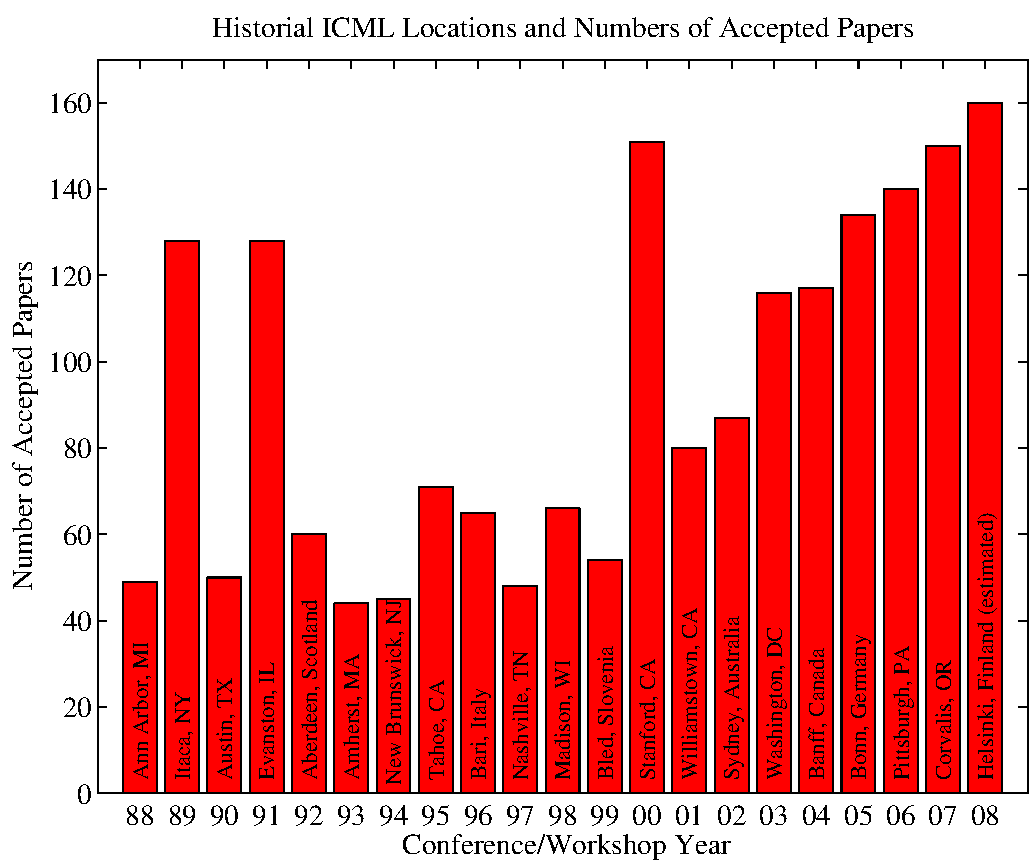
\includegraphics[width=\columnwidth]{icml_numpapers}}
\caption{Historical locations and number of accepted papers for International
  Machine Learning Conferences (ICML 1993 -- ICML 2008) and
  International Workshops on Machine Learning (ML 1988 -- ML
  1992). At the time this figure was produced, the number of
  accepted papers for ICML 2008 was unknown and instead estimated.}
\label{icml-historical}
\end{center}
\vskip -0.2in
\end{figure}

\subsection{Figures}

You may want to include figures in the paper to help readers visualize
your approach and your results. Such artwork should be centered,
legible, and separated from the text. Lines should be dark and at
least 0.5~points thick for purposes of reproduction, and text should
not appear on a gray background. Figures should be placed
near their place of reference, rather than at the end of the document.

Label all distinct components of each figure. If the figure takes the
form of a graph, then give a name for each axis and include a legend
that briefly describes each curve. Do not include a title inside the
figure; instead, the caption should serve this function.

Number figures sequentially, placing the figure number and caption
{\it after\/} the graphics, with at least 0.1~inches of space before
the caption and 0.1~inches after it, as in
Figure~\ref{icml-historical}.  The figure caption should be set in
9~point type and centered unless it runs two or more lines, in which
case it should be flush left.  You may float figures to the top or
bottom of a column, and you may set wide figures across both columns
(use the environment {\tt figure*} in \LaTeX), but always place
two-column figures at the top or bottom of the page.

\subsection{Algorithms}

If you are using \LaTeX, please use the ``algorithm'' and ``algorithmic''
environments to format pseudocode. These require
the corresponding stylefiles, algorithm.sty and
algorithmic.sty, which are supplied with this package.
Algorithm~\ref{alg:example} shows an example.

\begin{algorithm}[tb]
   \caption{Bubble Sort}
   \label{alg:example}
\begin{algorithmic}
   \STATE {\bfseries Input:} data $x_i$, size $m$
   \REPEAT
   \STATE Initialize $noChange = true$.
   \FOR{$i=1$ {\bfseries to} $m-1$}
   \IF{$x_i > x_{i+1}$}
   \STATE Swap $x_i$ and $x_{i+1}$
   \STATE $noChange = false$
   \ENDIF
   \ENDFOR
   \UNTIL{$noChange$ is $true$}
\end{algorithmic}
\end{algorithm}

\subsection{Tables}

You may also want to include tables that summarize material. Like
figures, these should be centered, legible, and numbered consecutively.
However, place the title {\it above\/} the table with at least
0.1~inches of space before the title and the same after it, as in
Table~\ref{sample-table}. The table title should be set in 9~point
type and centered unless it runs two or more lines, in which case it
should be flush left.

% Note use of \abovespace and \belowspace to get reasonable spacing
% above and below tabular lines.

\begin{table}[t]
\caption{Classification accuracies for naive Bayes and flexible
Bayes on various data sets.}
\label{sample-table}
\vskip 0.15in
\begin{center}
\begin{small}
\begin{sc}
\begin{tabular}{lcccr}
\hline
\abovespace\belowspace
Data set & Naive & Flexible & Better? \\
\hline
\abovespace
Breast    & 95.9$\pm$ 0.2& 96.7$\pm$ 0.2& $\surd$ \\
Cleveland & 83.3$\pm$ 0.6& 80.0$\pm$ 0.6& $\times$\\
Glass2    & 61.9$\pm$ 1.4& 83.8$\pm$ 0.7& $\surd$ \\
Credit    & 74.8$\pm$ 0.5& 78.3$\pm$ 0.6&         \\
Horse     & 73.3$\pm$ 0.9& 69.7$\pm$ 1.0& $\times$\\
Meta      & 67.1$\pm$ 0.6& 76.5$\pm$ 0.5& $\surd$ \\
Pima      & 75.1$\pm$ 0.6& 73.9$\pm$ 0.5&         \\
\belowspace
Vehicle   & 44.9$\pm$ 0.6& 61.5$\pm$ 0.4& $\surd$ \\
\hline
\end{tabular}
\end{sc}
\end{small}
\end{center}
\vskip -0.1in
\end{table}

Tables contain textual material that can be typeset, as contrasted
with figures, which contain graphical material that must be drawn.
Specify the contents of each row and column in the table's topmost
row. Again, you may float tables to a column's top or bottom, and set
wide tables across both columns, but place two-column tables at the
top or bottom of the page.
\subsection{Equations}
Your paper should contain several equations to define any mathematical terms.
For example, you may want to define a voting scheme for $k$-nearest neighbors
for a test example $x_i$ with nearest neighbors $knn$:
\begin{equation}
  p_i = \arg\max_c \sum_{\{x_j,y_j\} \in knn} I(y_j = c) \times \frac{1}{1+dist(x_j, x_i)}
\end{equation}\label{eqn:vote}

or the Silhouette Index $S$ of a clustering algorithm:
\begin{equation}
S = \frac{1}{K} \sum_{j=1}^{K}\frac{1}{|c_j|}\sum_{x_i \in c_j}s(x_i)
\end{equation}\label{eqn:silhouette}

\subsection{Citations and References}

Please use APA reference format regardless of your formatter
or word processor. If you rely on the \LaTeX\/ bibliographic
facility, use {\tt natbib.sty} and {\tt icml2014.bst}
included in the style-file package to obtain this format.

Citations within the text should include the authors' last names and
year. If the authors' names are included in the sentence, place only
the year in parentheses, for example when referencing Arthur Samuel's
pioneering work \yrcite{Samuel59}. Otherwise place the entire
reference in parentheses with the authors and year separated by a
comma \cite{Samuel59}. List multiple references separated by
semicolons \cite{kearns89,Samuel59,mitchell80}. Use the `et~al.'
construct only for citations with three or more authors or after
listing all authors to a publication in an earlier reference \cite{MachineLearningI}.

Authors should cite their own work in the third person
in the initial version of their paper submitted for blind review.
Please refer to Section~\ref{author info} for detailed instructions on how to
cite your own papers.

Use an unnumbered first-level section heading for the references, and
use a hanging indent style, with the first line of the reference flush
against the left margin and subsequent lines indented by 10 points.
The references at the end of this document give examples for journal
articles \cite{Samuel59}, conference publications \cite{langley00}, book chapters \cite{Newell81}, books \cite{DudaHart2nd}, edited volumes \cite{MachineLearningI},
technical reports \cite{mitchell80}, and dissertations \cite{kearns89}.

Alphabetize references by the surnames of the first authors, with
single author entries preceding multiple author entries. Order
references for the same authors by year of publication, with the
earliest first. Make sure that each reference includes all relevant
information (e.g., page numbers).


\section*{Acknowledgments}


Place acknowledgements in an unnumbered section at the
end of the paper. Typically, this will include
to colleagues who contributed to the ideas, individuals who
reviewed your submission, or external sources who helped
acquire data.


% In the unusual situation where you want a paper to appear in the
% references without citing it in the main text, use \nocite
\nocite{langley00}

\bibliography{example}
\bibliographystyle{icml2014}

\end{document}


% This document was modified from the file originally made available by
% Pat Langley and Andrea Danyluk for ICML-2K. This version was
% created by Lise Getoor and Tobias Scheffer, it was slightly modified
% from the 2010 version by Thorsten Joachims & Johannes Fuernkranz,
% slightly modified from the 2009 version by Kiri Wagstaff and
% Sam Roweis's 2008 version, which is slightly modified from
% Prasad Tadepalli's 2007 version which is a lightly
% changed version of the previous year's version by Andrew Moore,
% which was in turn edited from those of Kristian Kersting and
% Codrina Lauth. Alex Smola contributed to the algorithmic style files.
